\section{Stable systems}

For stationary processes resulting from filtering white noise through a stable dynamical system, the spectrum can be calculated using the transfer function.
Let's consider the process $y(\cdot)$ obtained by filtering an input process $u(\cdot)$ through an asymptotically stable dynamical system described by transfer function $W(z)$. 
The spectra of the two processes are related by the equation:
\[\Gamma_{yy}(\omega)=\left\lvert W(e^{j\omega})\right\rvert^2\Gamma_{uu}(\omega)\]

Given that the expected value of $u(\cdot)$ is zero, applying the convolution formula reveals that $y(\cdot)$ also has a null expectation.
To compute the input-output cross-covariance function, we start with the convolution formula:
\[y(t_2)=\sum_{i=0}^\infty w(i)u(t_2-i)\]
Multiplying both sides by $u(t_1)$ yields:
\[u(t_1)y(t_2)=u(t_1)\sum_{i=0}^{\infty}w(i)u(t_2-i)=\sum_{i=0}^\infty w(i)u(t_1)u(t_2-i)\]
Taking the expected value of both sides, we obtain:
\[\mathbb{E}\left[u(t_1)y(t_2)\right]=\mathbb{E}\left[u(t_1)\sum_{i=0}^{\infty}w(i)u(t_2-i)\right]=\sum_{i=0}^\infty w(i) \mathbb{E}\left[u(t_1)u(t_2-i)\right]\]
This leads to:
\[\gamma_{uy}(t_1,t_2)=\sum_{i=0}^\infty w(i)\gamma_{uu}(t_1,t_2-i)\]
Similarly, multiplying both sides of the convolution formula by $y(t_1)$ gives:
\[y(t_1)y(t_2)=y(t_1)\sum_{i=0}^{\infty}w(i)u(t_2-i)=\sum_{i=0}^\infty w(i)y(t_1)u(t_2-i)\]
Taking the expectation leads to:
\[\gamma_{yy}(t_1,t_2)=\sum_{i=0}^\infty w(i)\gamma_{yu}(t_1,t_2-i)\]
For stationary processes, these auto-covariance and cross-covariance functions depend only on the difference between the two temporal indices $\tau = t_2-t_1$:
\[\begin{cases}
    \gamma_{uy}(\tau)=\sum_{i=0}^\infty w(i)\gamma_{uu}(\tau-i) \\
    \gamma_{yy}(\tau)=\sum_{i=0}^\infty w(i)\gamma_{yu}(\tau-i)
\end{cases}\]
Let's introduce the (bilateral) Z-transforms of these covariance functions:
\[\Phi_{uu}(z)=\sum_{-\infty}^{+\infty}\gamma_{uu}(\tau)z^{-\tau} \qquad \Phi_{yy}(z)=\sum_{-\infty}^{+\infty}\gamma_{yy}(\tau)z^{-\tau} \qquad \Phi_{uy}(z)=\sum_{-\infty}^{+\infty}\gamma_{uy}(\tau)z^{-\tau}\]
These transforms are useful because they allow us to compute the power spectral densities of the input and output, as well as the cross-spectrum, by simply applying $z=e^{j\omega}$:
\[\Gamma_{uu}(\omega)=\Phi_{uu}(e^{j\omega}) \qquad \Gamma_{yy}(\omega)=\Phi_{yy}(e^{j\omega}) \qquad \Gamma_{uy}(\omega)=\Phi_{uy}(e^{j\omega})\]
It's worth noting that while $\Gamma_{uu}(\omega)=\Phi_{uu}(e^{j\omega})$ and $\Gamma_{yy}(\omega)=\Phi_{yy}(e^{j\omega})$ are real functions, the input-output cross spectrum can be complex. 
Additionally, since $\gamma_{uy}(\tau)=\gamma_{yu}(-\tau)$, we have:
\[\Phi_{yu}(z)=\Phi(z^{-1})\rightarrow\Gamma_{yu}(\omega)=\Gamma_{uy}(\omega)^\ast\]
Here, $\ast$ denotes the complex conjugate.
By performing Z-transforms on the expressions for $\gamma_{uy}(\cdot)$ and $\gamma_{yy}(\cdot)$, and recalling the properties of Z-transforms, specifically:
\begin{itemize}
    \item The Z-transform of the convolution product is equal to the product of the transforms of the two processes.
    \item The Z-transform of the impulse response $w(\cdot)$ is the transfer function of the system.
\end{itemize}
We arrive at:
\[\gamma_{uy}(\tau)=\sum_{i=0}^{\infty}w(i)\gamma_{uu}(\tau-i)\rightarrow\Phi_{uy}(z)=W(z)\Phi_{uu}(z)\]
\[\gamma_{yy}(\tau)=\sum_{i=0}^{\infty}w(i)\gamma_{yu}(\tau-i)\rightarrow\Phi_{yy}(z)=W(z)\Phi_{yu}(z)\]
Expanding these expressions yields:
\[\Phi_{yy}(z)=W(z)\Phi_{yu}(z)=W(z)\Phi_{uy}(z^{-1})=W(z)W(z^{-1})\Phi_{uu}(z^{-1})\]
Finally, since $\Phi_{uu}(z^{-1})=\Phi_{uu}(z)$, we also have:
\[\Phi_{yy}(z)=W(z)W(z^{-1})\Phi_{uu}(z)\]
To obtain the power spectral density, we simply substitute $z = e^{j\omega}$:
\[\Gamma_{yy}(\omega)=\left\lvert W(e^{j\omega})\right\rvert^2\lambda^2 \]

\subsection{MA(1) spectrum}
To compute the spectrum of an MA(1) process, we utilize the direct definition, leveraging the property that the auto-correlation function is zero for lags greater than 1:
\begin{align*}
    \Gamma(\omega)  &= \sum_{\tau=-\infty}^\infty\tilde{\gamma(\tau)}e^{-j\omega\tau} \\
                    &= \tilde{\gamma}(0) + \tilde{\gamma}(1)e^{-j\omega}+\tilde{\gamma}(-1)e^{j\omega} \\
                    &= \tilde{\gamma}(0) +2\tilde{\gamma}(1)\dfrac{e^{j\omega}+e^{-j\omega}}{2} \\
                    &= \tilde{\gamma}(0) +2\tilde{\gamma}(1)\cos(\omega) \\
                    &= \left(1+c^2+2c\cos(\omega)\right)\lambda^2
\end{align*}
Alternatively, we can employ the transfer function $W(z) = 1 + cz^{-1}$ to compute the complex spectrum:
\[\Phi_{vv}(z)=W(z)W(z^{-1})\Phi_{\eta\eta}(z)=(1+cz^{-1})(1+cz)\lambda^2=\left(1+c^2+2c\cos(\omega)\right)\lambda^2\]
As a result, we have: 
\[\Gamma(\omega)=\Phi_{vv}(e^{j\omega})=\left(1+c^2+2c\cos(\omega)\right)\lambda^2\]
The spectrum shape varies with the value of parameter $c$: 
\begin{itemize}
    \item $c>0$: realizations tend to maintain the sign between consecutive times, with low frequencies dominating.
    \item $c<0$: opposite behavior occurs, with high frequencies dominating.
\end{itemize}

\begin{figure}[H]
    \centering
    \begin{subfigure}{0.49\textwidth}
        \centering
        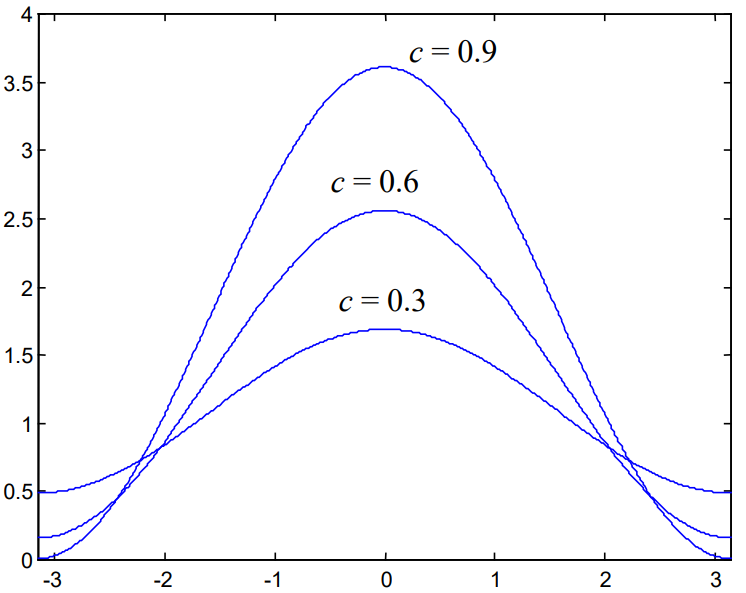
\includegraphics[width=0.6\linewidth]{images/cp.png} 
        \caption{Positive}
    \end{subfigure}
    \begin{subfigure}{0.49\textwidth}
        \centering
        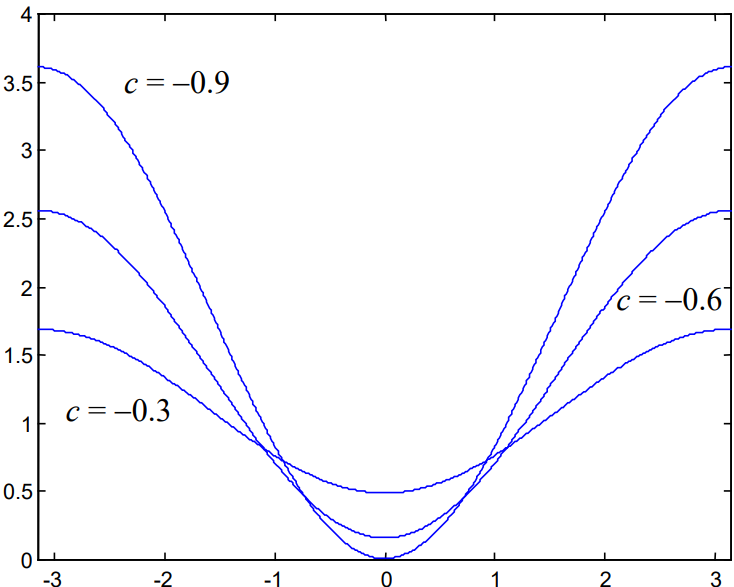
\includegraphics[width=0.6\linewidth]{images/cn.png}
        \caption{Negative}
    \end{subfigure}
    \caption{Possible sign for the constant $c$}
\end{figure}
We can also deduce the process variance from the spectrum:
\begin{align*}
    \gamma(0)   &= \tilde{\gamma}(0) \\
                &= \dfrac{1}{2\pi}\int_{-\pi}^{\pi}\Gamma(\omega)d\omega \\
                &= \dfrac{1}{2\pi}\int_{-\pi}^{\pi}\left(1+c^2+2c\cos(\omega)\right)\lambda^2d\omega \\
                &= \left(1+c^2\right)\lambda^2 \dfrac{1}{2\pi}\int_{-\pi}^{\pi}d\omega+ 2c\lambda^2\dfrac{1}{2\pi}\int_{-\pi}^{\pi}\cos(\omega)d\omega \\
                &= \left(1+c^2\right)\lambda^2 + 2c\lambda^2\dfrac{1}{2\pi}\left[\sin(\omega)\right]^{\pi}_{-\pi} \\
                &= \left(1+c^2\right)\lambda^2
\end{align*}

\subsection{AR(1) spectrum}
Now, let's examine an AR(1) process:
\[v(t)=av(t-1)+\eta(t)\]
Here, $\eta(\cdot)$ follows a white noise distribution $WN(0,\lambda^2)$ with $\left\lvert a \right\rvert < 1$. 
The transfer function of this process is:
\[W(z)=\dfrac{1}{1-az^{-1}}\]
The power spectral density can be computed as follows:
\[\Phi_{vv}(z)=W(z)W(z^{-1})\Phi_{\eta\eta}(z)=\dfrac{1}{\left( 1-az^{-1} \right)\left( 1-az \right)}\lambda^2=\dfrac{1}{1+a^2-a(z+z^{-1})}\lambda^2\]
And the spectral density at frequency $\omega$ is given by:
\[\Gamma(\omega)=\Phi_{vv}(e^{j\omega})=\dfrac{1}{1+a^2-a\cos(\omega)}\lambda^2\]
The spectrum exhibits a markedly different shape depending on the sign of $a$.
Specifically:
\begin{itemize}
    \item For $a>0$, most of the frequency content concentrates at low frequencies.
    \item Conversely, for $a<0$, the opposite trend occurs.
\end{itemize}
This difference is visually represented in the following figure. 
\begin{figure}[H]
    \centering
    \begin{subfigure}{0.49\textwidth}
        \centering
        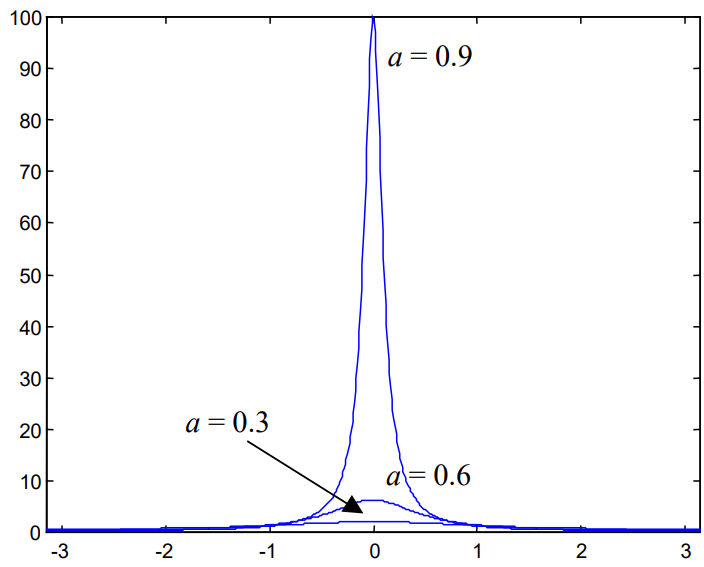
\includegraphics[width=0.6\linewidth]{images/ap.png} 
        \caption{Positive}
    \end{subfigure}
    \begin{subfigure}{0.49\textwidth}
        \centering
        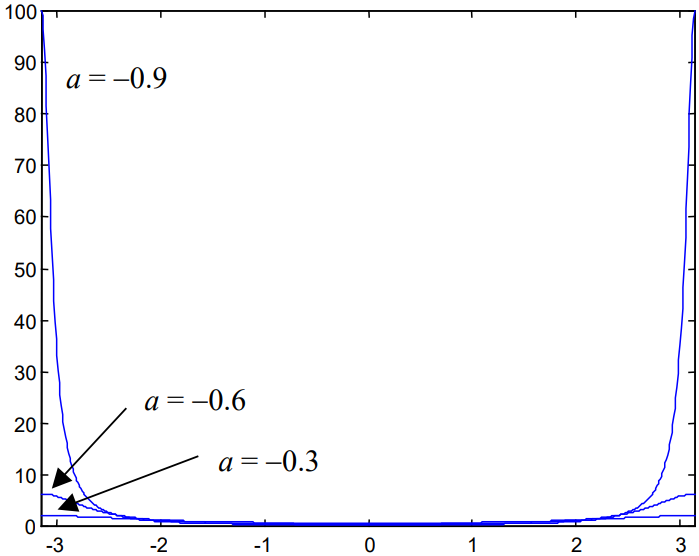
\includegraphics[width=0.6\linewidth]{images/an.png}
        \caption{Negative}
    \end{subfigure}
    \caption{Possible sign for the constant $a$}
\end{figure}

\subsection{ARMA(1,1) spectrum}
Let's now examine the ARMA(1, 1) process with $\left\lvert a \right\rvert  < 1$:
\[v(t)=av(t-1)+\eta(t)+c\eta(t-1)\]
Here, $\eta(\cdot)$ follows a white noise distribution $WN(0,\lambda^2)$. 
The transfer function is given by:
\[W(z)=\dfrac{1+cz^{-1}}{1-az^{-1}}\]
The power spectral density can then be computed as:
\[\Phi(z)=W(z)W(z^{-1})\lambda^2=\dfrac{\left(1+cz^{-1}\right)\left(1+cz\right)}{\left(1-az^{-1}\right)\left(1-az\right)}\lambda^2=\dfrac{1+c^2+c(z+z^{-1})}{1+a^2-a(z+z^{-1})}\lambda^2\]
And the spectral density at frequency $\omega$ is expressed as:
\[\Gamma(\omega)=\Phi(e^{j\omega})=\dfrac{1+c^2+2c\cos(\omega)}{1+a^2-2a\cos(\omega)}\lambda^2\]